\documentclass[10]{article}
\usepackage[titletoc, title]{appendix}
\usepackage{graphicx}
\usepackage{pdfpages}
%opening
\title{Software Design Document}
\author{Michael Farghali}

\begin{document}

\maketitle



\section*{Introduction}
This is a preliminary Software Design Document (SSD) for my mini-Pascal complier that I will be working on over the next two semesters. When completed it should accept a text file which represents a mini pascal language. The text file should then be able to be converted to assembly language if its syntax is correct according to our production rules. 
\section*{Scanner}
The Scanner class should read in a file and process it character by character. It is based on a Deterministic Finite Automata, Appendix A, and the given grammars. The Scanner reads in a file and attempts to match each string to a given keyword, symbol, or number. It returns a valid Token if the string is valid in the language or it will return false. See Appendix B for list of valid Tokens.

\section*{Parser}
The Parser class processes a text file token by token which are given by the Scanner class. It uses the grammar rules listed in Appendix C to match the tokens against expected tokens. It will eventually create a parse tree but for now it only checks that the production rules are followed. 


\newpage
\begin{appendices}
\section{Deterministic Finite Automata}
\begin{figure}[!ht]
	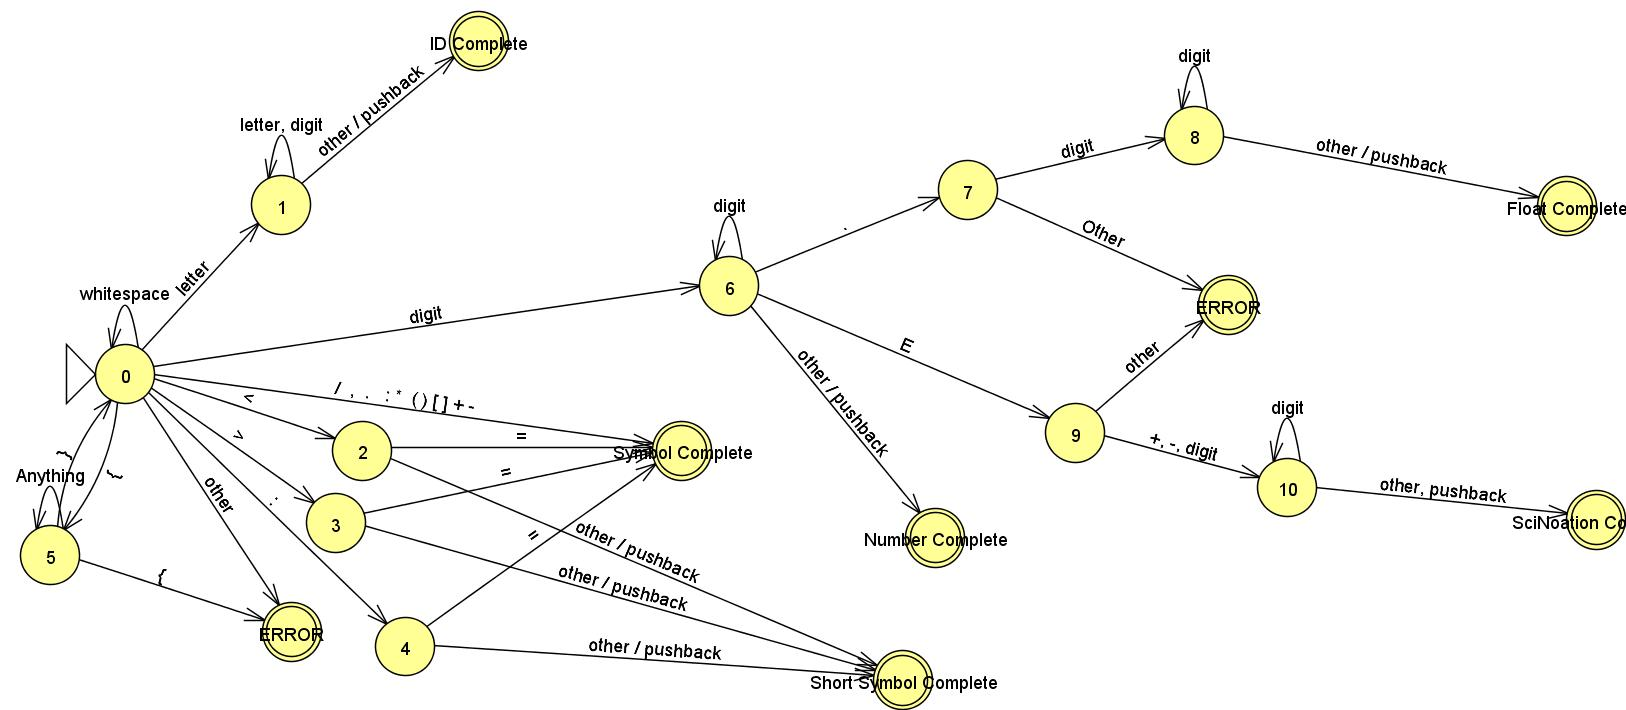
\includegraphics[width=\textwidth]{ScannerDFA.jpg}
\end{figure}
\section{List of Keywords}
Symbols: $ . , - + * / ( ) { } [ ] { } < <= > >= : := ;$  
\newline
Keywords: div, mod, and, program, id, var, array, of, num, integer, real, function, procedure, begin, end, if, then, else, while, do, not
\section{Grammar Rules}
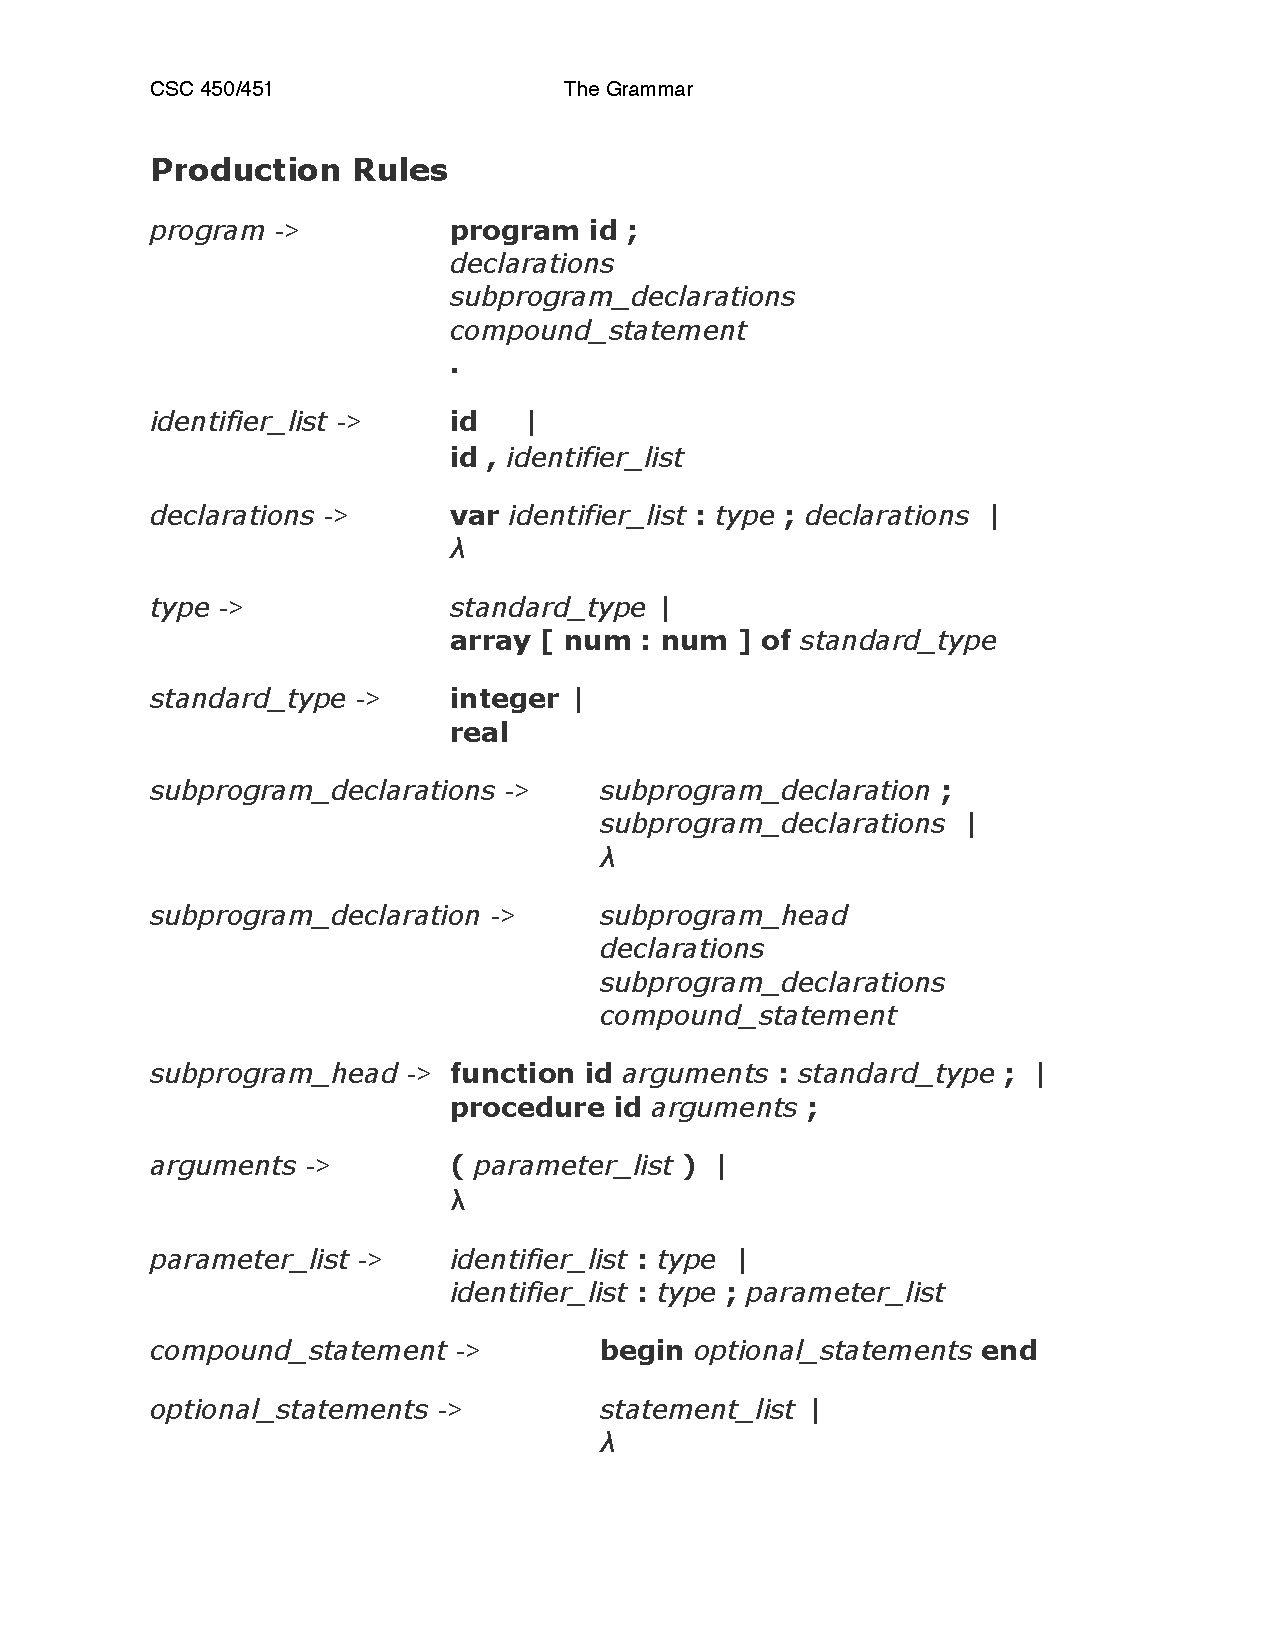
\includepdf[pages=-, scale=.8, noautoscale = true]{Grammar.pdf}
\end{appendices}


\end{document}
